% IEEE Conference-style Thesis
% Compile: pdflatex thesis_final.tex && pdflatex thesis_final.tex
\documentclass[conference]{IEEEtran}

% ---- Packages ----
\usepackage{cite}
\usepackage{amsmath,amssymb,amsfonts}
\usepackage{algorithmic}
\usepackage{graphicx}
\usepackage{stfloats}    % Better float placement in two-column mode
\usepackage{placeins}    % \FloatBarrier to anchor figures near text
\usepackage{textcomp}
\usepackage{xcolor}
\usepackage{booktabs}
\usepackage{multirow}
\usepackage{hyperref}
\usepackage{url}
\usepackage{tikz}
\usepackage{pgfplots}
\pgfplotsset{compat=1.18}
\usetikzlibrary{shapes.geometric, arrows.meta, positioning, fit, backgrounds, calc, patterns, decorations.pathreplacing}
\graphicspath{{images/}}

\renewcommand{\arraystretch}{1.15}

% TikZ styles
\tikzset{
    block/.style={rectangle, draw, fill=blue!8, text width=2.2cm, text centered, rounded corners, minimum height=0.8cm, font=\footnotesize},
    blockwide/.style={rectangle, draw, fill=blue!8, text width=3.0cm, text centered, rounded corners, minimum height=0.8cm, font=\footnotesize},
    sensor/.style={rectangle, draw, fill=green!15, text width=1.8cm, text centered, rounded corners, minimum height=0.7cm, font=\footnotesize},
    model/.style={rectangle, draw, fill=orange!20, text width=2.4cm, text centered, rounded corners, minimum height=0.8cm, font=\footnotesize},
    output/.style={rectangle, draw, fill=red!12, text width=2.2cm, text centered, rounded corners, minimum height=0.8cm, font=\footnotesize},
    arrow/.style={-Stealth, thick},
    dashedarrow/.style={-Stealth, thick, dashed},
    layerbox/.style={draw, dashed, rounded corners, inner sep=6pt},
}

\begin{document}

\title{Edge-RL: Autonomous Post-Harvest Ripening Control via Distilled Reinforcement Learning on the Edge}

\author{
\IEEEauthorblockN{Tristan O. Jadman}
\IEEEauthorblockA{
Department of Computer Engineering\\and Mechatronics \\
\textit{Undergraduate Thesis}}
\and
\IEEEauthorblockN{Engr. Francis Jann Alagon}
\IEEEauthorblockA{
Department of Computer Engineering\\and Mechatronics \\
\textit{Thesis Adviser}}
}

\maketitle

% ==============================================================
\begin{abstract}
Post-harvest losses account for 20--40\% of tomato production in developing countries, driven by the absence of affordable, intelligent decision-support systems. Existing IoT solutions provide passive monitoring without autonomous action, while cloud-based reinforcement learning (RL) systems require expensive infrastructure and continuous connectivity. This thesis proposes \textit{Edge-RL}, a novel system that deploys a complete RL-based decision pipeline---from visual perception to autonomous ripening control---entirely on a \$33 ESP32-S3 microcontroller. The system extracts a Continuous Chromatic Index from RGB statistics via a MobileNetV2-based feature extractor and feeds a state vector to a distilled Deep Q-Network policy. By leveraging ESP-DL's hardware-optimized inference, Edge-RL achieves sub-2-second combined inference for spectral feature extraction and control decisions. Hardware-level safety guardrails enforce biological temperature constraints ($12.5$--$35^{\circ}$C) independent of the learned policy. This work presents the first demonstration of a complete sim-to-edge RL pipeline for agricultural post-harvest optimization.
\end{abstract}

\begin{IEEEkeywords}
Edge intelligence, reinforcement learning, post-harvest management, ESP32-S3, sim-to-real transfer, model compression, continuous chromatic index, digital twin
\end{IEEEkeywords}

% ==============================================================
% Chapters
% ==============================================================

\section{Introduction}
\label{ch:introduction}

\subsection{Background of the Study}
The Philippines, despite being an agricultural nation, faces significant challenges in post-harvest management. High-value crops like tomatoes (\textit{Solanum lycopersicum}) suffer post-harvest losses estimated at 20--40\%, primarily due to poor handling, lack of cold chain infrastructure, and inadequate storage facilities \cite{fao2019}. Unlike grain crops, tomatoes are climacteric fruits that continue to respire and ripen after harvest, making temperature control critical for extending shelf life and ensuring market viability.

Commercial operations mitigate these losses using industrial ripening chambers equipped with precise climate control systems. These facilities use ethylene gas injection and active refrigeration to synchronize ripening, ensuring uniform quality for supermarkets. However, the capital expenditure for such infrastructure ranges from \$10,000 to \$50,000 \cite{prasad2018}, effectively excluding the 5.5 million smallholder farming households in the Philippines who typically earn less than \$2,000 annually. As a result, small farmers are forced to sell their produce immediately after harvest at fluctuating farm-gate prices, often leading to income instability and food waste.

\subsection{Statement of the Problem}
Smallholder tomato farmers lack access to affordable, intelligent post-harvest decision-support systems. Existing solutions fall into two extremes: passive monitoring tools (IoT sensors) that provide data but no actionable control, and high-end industrial systems that are cost-prohibitive. Cloud-based Reinforcement Learning (RL) solutions have shown promise in controlled environment agriculture but require continuous internet connectivity, which is unreliable or absent in many rural Philippine farming communities. There is currently no standalone, low-cost system capable of autonomous, optimal ripening control at the edge.

\subsection{Objectives of the Study}
This study aims to develop "Edge-RL," a standalone autonomous ripening control system running on a low-cost microcontroller.

\subsubsection{General Objective}
To develop a low-cost, offline Reinforcement Learning system on an ESP32-S3 microcontroller that optimizes the post-harvest ripening of tomatoes by balancing quality preservation with energy efficiency.

\subsubsection{Specific Objectives}
\begin{enumerate}
    \item To design a low-cost, standalone ripening chamber hardware (BOM $<$ \$50) integrating an ESP32-S3, camera, and relay-controlled heating element.
    \item To implement a Deep Q-Network (DQN) policy trained in a physics-based digital twin that generalizes across tomato cultivars using domain randomization.
    \item To validate the system's performance by distilling the policy to an edge-optimized model (INT8) and achieving a harvest timing error of less than 20\% in sim-to-real transfer.
\end{enumerate}

\subsection{Significance of the Study}

This study addresses the critical issue of post-harvest loss, which accounts for up to 42\% of fruit and vegetable production globally according to the FAO \cite{fao2019}. In developing economies like the Philippines, these losses are exacerbated by the lack of cold chain infrastructure, often forcing smallholder farmers to sell produce at low prices or face total spoilage \cite{worldbank2020}.

By developing a low-cost, intelligent ripening chamber, this research directly benefits:
\begin{itemize}
    \item \textbf{Smallholder Farmers:} Providing a tool to control the timing of produce sales, decoupling harvest time from market saturation.
    \item \textbf{Agricultural Logistics:} Reducing spoilage during transport \cite{kader2005} through precise biological control.
    \item \textbf{Technological Advancement:} Demonstrating the feasibility of deploying advanced Reinforcement Learning on \$2 microcontrollers (Edge AI) for complex biological systems \cite{warden2019tinyml}.
\end{itemize}

\subsection{Scope and Limitations}

\subsubsection{Scope}
This thesis encompasses the complete pipeline from simulation-based RL training to on-device inference on embedded hardware. The following boundaries define the system's scope:

\begin{enumerate}
    \item \textbf{Single-Fruit Focus:} The system monitors and controls the ripening of a single tomato unit within an enclosed chamber. This isolates the ripening kinetics of one fruit and avoids the complexity of batch effects such as inter-fruit ethylene signaling.

    \item \textbf{Heater-Only Actuation:} The control mechanism is limited to a resistive heating element (raising temperature above ambient) and passive ventilation (cooling toward ambient). No active refrigeration (compressor or Peltier element) is used, constraining the controllable temperature range to $T_{\text{ambient}} \le T_{\text{chamber}} \le 35^\circ$C.

    \item \textbf{Target Crop:} The ripening model is calibrated for Philippine tomato varieties, specifically the commercial hybrid ``Diamante Max F1'' and native ``Kamatis Tagalog.'' The ripening rate constant $k_1$ is parameterized to reflect the kinetics of these cultivars.

    \item \textbf{Offline Edge Deployment:} All inference and control logic execute locally on the ESP32-S3 microcontroller. No cloud connectivity is required during operation; the system is designed for rural areas without reliable internet access.

    \item \textbf{Sim-to-Edge Pipeline:} The study validates the complete pipeline from Gymnasium-based environment simulation, through DQN teacher training and student distillation, to pure-C inference on the Xtensa LX7 core.

    \item \textbf{State-Space Ablation:} Three observation variants are evaluated (7D scalar, 16D with RGB statistics, 20D with spatial pooling) to determine the optimal state representation for edge deployment.
\end{enumerate}

\subsubsection{Limitations}
The following limitations constrain the generalizability and completeness of the current work:

\begin{enumerate}
    \item \textbf{Simulation-Only Training:} The RL policy is trained entirely in a physics-based digital twin. While domain randomization is applied to improve robustness, the policy has not been validated against real physical tomatoes in a closed-loop setting.

    \item \textbf{Simulated Colour Statistics:} The RGB colour statistics (mean, standard deviation, mode) used in Variant B and C are generated synthetically by the simulator. Real camera-derived statistics may exhibit different noise characteristics, lens distortion, and lighting dependencies.

    \item \textbf{No Active Cooling:} The absence of a compressor or Peltier module means the system cannot cool below ambient temperature. In tropical climates where $T_{\text{ambient}}$ may exceed 30$^\circ$C, the agent's ability to slow ripening is fundamentally limited to the MAINTAIN action.

    \item \textbf{No Ethylene Sensing:} The system does not incorporate ethylene gas sensors, which provide a direct biochemical indicator of climacteric ripening onset. Ripeness estimation relies solely on visual (RGB) and environmental (temperature, humidity) features.

    \item \textbf{Fixed Policy Architecture:} The student MLP architecture (64$\times$64, ReLU) is fixed at compile time. On-device fine-tuning or continual learning is not supported in the current firmware; the policy is static after deployment.

    \item \textbf{Single-Cultivar ODE:} The ripening ODE uses a single $k_1$ constant per episode. Real-world cultivar variability within a batch is not captured, and the model does not account for fruit maturity at harvest or mechanical damage.
\end{enumerate}


\subsection{Definition of Terms}
\begin{description}
    \item[Edge-RL] The proposed system architecture where Reinforcement Learning inference occurs directly on the edge device (microcontroller) rather than in the cloud.
    \item[Climacteric Fruit] Fruits that exhibit a spike in respiration and ethylene production during ripening (e.g., tomato, banana, mango).
    \item[Knowledge Distillation] A compression technique where a small "student" model learns to mimic the output of a larger "teacher" model.
    \item[Continuous Chromatic Index ($X$)] A computed scalar value derived from the spectral reflectance of the fruit, representing its ripeness stage on a continuous scale from Green ($X=1$) to Red ($X=0$).
\end{description}

\chapter{Review of Related Literature}
\label{ch:rrl}

\section{Post-Harvest Characteristics of Philippine Tomato Varieties}
Understanding the specific biological kinetics of local tomato cultivars is essential for calibrating the physics-based digital twin. In the Philippines, the market is dominated by two primary categories: commercial F1 hybrids and native cultivars.

\subsection{Diamante Max F1}
"Diamante Max" is widely favored by commercial growers in the Philippines due to its heat tolerance and high yield potential. However, studies indicate it is a highly perishable variety characterized by high moisture content ($\approx$95.31\%) and relatively thin skin \cite{diamante_properties}. Under ambient tropical conditions (23--34$^\circ$C), the fruit undergoes rapid physicochemical changes, with shelf life often limited to 14 days without intervention \cite{diamante_storage}.
Physiologically, it exhibits a classic climacteric respiratory peak. Research by the Postharvest Horticulture Training and Research Center (PHTRC) at UPLB suggests that while storage at 7--10$^\circ$C significantly delays ripening, such low temperatures are energy-intensive and risk chilling injury. The optimal storage for quality retention is often cited at 13--15$^\circ$C \cite{uplb_phtrc}, aligning with the proposed system's target control range.

\subsection{Native "Tagalog" Cultivars}
Native cultivars, often referred to as "Kamatis Tagalog", are typically smaller, irregular in shape, and possess thinner pericarps compared to commercial hybrids. These varieties are highly valued for their sour flavor profile in traditional cuisine but suffer from even faster deterioration rates due to higher respiration and susceptibility to mechanical damage during transport \cite{native_tomato}. Their ripening kinetics ($k_1$) are generally higher than hybrids, requiring more aggressive cooling interventions to extend shelf life. This variability between "slow-ripening" hybrids and "fast-ripening" natives motivates the need for an adaptive control system (RL) rather than a fixed rule-based controller.

\section{Reinforcement Learning in Controlled Environment Agriculture}
Reinforcement Learning (RL) has emerged as a powerful tool for optimizing complex agricultural processes. Unlike Proportional-Integral-Derivative (PID) controllers which react to setpoint errors, RL agents can learn anticipatory strategies that optimize long-term rewards \cite{overweg2021cropgym}.

\subsection{Climate Control and Irrigation}
Chen \textit{et al.} demonstrated the efficacy of Deep Q-Networks (DQN) for greenhouse climate control \cite{chen2022greenhouse}, reducing energy consumption while maintaining optimal growth conditions. Similarly, Yang \textit{et al.} applied RL to precision irrigation \cite{yang2020irrigation}, and Hemming \textit{et al.} explored AI sensors for cherry tomatoes \cite{hemming2020greenhouse}. While effective, these systems typically rely on cloud interfaces or heavy compute servers \cite{ray2017}, which introduces latency and connectivity risks ill-suited for rural deployment \cite{prasad2018}.

\subsection{Post-Harvest Management}
Application of RL in post-harvest storage is less explored. Current systems largely rely on Model Predictive Control (MPC) or standard IoT monitoring \cite{li2021edgeai}. "Edge-RL" proposes shifting the computational burden to a one-time offline training phase, enabling the deployment of complex policies on resource-constrained devices like the ESP32.

\section{Edge AI and Model Compression}
Deploying deep learning models on microcontrollers (TinyML) requires aggressive optimization to fit within strict memory ($<$500 KB SRAM) and compute constraints.

\subsection{Knowledge Distillation}
Hinton \textit{et al.} introduced Knowledge Distillation, where a small "student" model is trained to mimic the soft outputs (logits) of a large "teacher" model \cite{hinton2015distilling}. In the context of RL, Policy Distillation \cite{ruffy2019distilling} allows a massive DQN (Teacher) to explore the environment and learn optimal Q-values, which are then compressed into a tiny MLP (Student) that creates a direct mapping from state to best action. This approach retains the "intelligence" of the large model while discarding parameters unnecessary for inference.

\subsection{Quantization and ESP-DL}
Standard 32-bit floating-point (FP32) models are too large and slow for the ESP32-S3. Quantization to 8-bit integers (INT8) reduces model size by 4$\times$ and accelerates inference by utilizing SIMD instructions (e.g., Xtensa LX7 vector extensions). The ESP-DL library \cite{espdl2024} provides optimized INT8 kernels that outperform generic interpreters like TensorFlow Lite for Microcontrollers (TFLite Micro) on Espressif chips. By combining Policy Distillation with INT8 Quantization, it is possible to execute complex control policies in $<$10ms on-device.

\section{Methodology}
\label{ch:methodology}

\subsection{System Architecture}
The Edge-RL system is designed as a closed-loop control system where a microcontroller (ESP32-S3) makes real-time decisions based on visual feedback from a camera and environmental data from sensors. The architecture consists of three main subsystems: the Perception Module, the Decision Engine (RL Policy), and the Actuation System.

\begin{figure}[htbp]
    \centering
    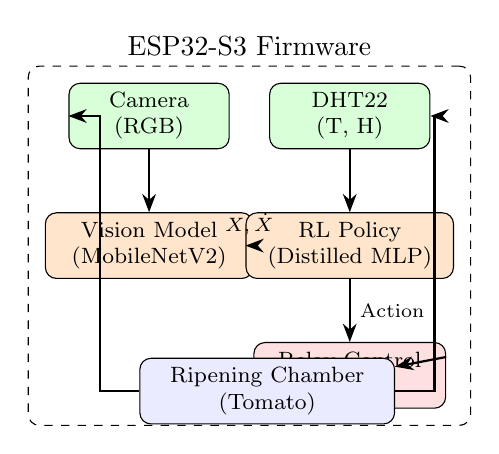
\begin{tikzpicture}[node distance=1.2cm, auto]
        % Nodes
        \node [sensor] (cam) {Camera (RGB)};
        \node [sensor, right=0.5cm of cam] (dht) {DHT22 (T, H)};
        \node [model, below=0.8cm of cam] (vision) {Vision Model\\(MobileNetV2)};
        \node [model, below=0.8cm of dht] (policy) {RL Policy\\(Distilled MLP)};
        \node [output, below=0.8cm of policy] (act) {Relay Control\\(Heater)};
        \node [blockwide, below=1.0cm of vision, xshift=1.5cm] (env) {Ripening Chamber\\(Tomato)};

        % Edges
        \draw [arrow] (env.west) -- ++(-0.5,0) |- (cam.west);
        \draw [arrow] (env.east) -- ++(0.5,0) |- (dht.east);
        \draw [arrow] (cam) -- (vision);
        \draw [arrow] (dht) -- (policy);
        \draw [arrow] (vision) -- node[above, font=\scriptsize] {$X, \dot{X}$} (policy);
        \draw [arrow] (policy) -- node[right, font=\scriptsize] {Action} (act);
        \draw [arrow] (act) -- (env);
        
        % Background box
        \begin{scope}[on background layer]
            \node [layerbox, fit=(cam) (dht) (vision) (policy) (act), label=above:ESP32-S3 Firmware] {};
        \end{scope}
    \end{tikzpicture}
    \caption{System Block Diagram. The ESP32-S3 handles both vision (Continuous Chromatic Index extraction) and control (RL inference). Sensors provide feedback from the physical chamber.}
    \label{fig:arch}
\end{figure}

The perception pipeline begins with the OV2640 camera capturing an RGB frame of the tomato at user-configurable intervals (default: every 30 minutes). A MobileNetV2 feature extractor, trained via transfer learning on a tomato ripeness dataset, computes a Continuous Chromatic Index $X \in [0, 1]$. A DHT22 sensor provides chamber temperature $T$ and relative humidity $H$. These readings, combined with temporal signals (elapsed time $t_e$ and remaining time $t_{\text{rem}}$), form the state vector $S_t$ fed to the RL policy.

Classification accuracy is evaluated using per-class precision, recall, F1-score, and a confusion matrix. The target is $\geq$85\% top-1 accuracy on held-out test images, comparable to similar deep learning approaches for tomato ripeness classification \cite{zhang2021tomato, phan2023tomato}. Transfer learning effectiveness is quantified through an ablation study: (i)~training from scratch, (ii)~ImageNet pre-training only, and (iii)~pre-training + fine-tuning on real tomato images.

\subsection{Digital Twin Construction}
To overcome the data inefficiency of RL, we constructed a physics-based digital twin that models the ripening kinetics of the tomato. The simulator faithfully reproduces the thermal dynamics of the physical ripening chamber and the biological response of the fruit.

\subsubsection{Ripening Dynamics (ODE)}
We model the ripening process using a first-order Ordinary Differential Equation (ODE) derived from Arrhenius kinetics. The Continuous Chromatic Index ($X \in [0, 1]$) represents the ripeness state, where $X=1$ is Green and $X=0$ is Red. The rate of change $\frac{dX}{dt}$ is governed by temperature $T$:

    \noindent In an increasing frequency along the visible spectrum, the range proceeds from Red to Green (ROYG). Thus, $X$ maps directly to this spectral ordering: high $X$ corresponds to the green end and low $X$ to the red end.  X is derived from the mean RGB statistics of the tomato ROI by mapping the ROYG spectral shift to a peak-wavelength intensity ratio.  Unlike the 0--5 USDA staging \cite{usda1991} that discretizes a continuous process, $X$ preserves the full gradient of color change, enabling proportional control and fine-grained reward shaping.

\begin{equation}
    \frac{dX}{dt} = -k_1 (T - T_{base}) X
    \label{eq:ode_ripening}
\end{equation}

where:
\begin{itemize}
    \item $k_1$: Cultivar-specific ripening rate constant (calibrated to $\approx 0.08$ day $^{-1} {^\circ}\text{C}^{-1}$ for Diamante Max).
    \item $T_{base}$: Base temperature below which ripening effectively stops ($12.5^\circ$C).
    \item $T$: Current chamber temperature ($^\circ$C).
\end{itemize}

\subsubsection{Thermal Model}
The chamber temperature $T$ acts as the control variable. Since the system uses a heater-only configuration with passive cooling, the temperature dynamics are modeled as:
\begin{equation}
    T_{t+1} = T_t + \Delta u \cdot \text{Action} + k_{loss}(T_{amb} - T_t)
\end{equation}
where $k_{loss}$ represents thermal leakage to the ambient environment $T_{amb}$.

\subsubsection{Domain Randomization}
To ensure the RL policy generalizes beyond the nominal simulator parameters, the digital twin applies domain randomization at each episode reset. This forces the agent to learn robust strategies rather than overfitting to a single set of physics.

\begin{table}[htbp]
\caption{Domain Randomization Parameters}
\label{tab:domain_rand}
\centering
\begin{tabular}{@{}llc@{}}
\toprule
\textbf{Parameter} & \textbf{Distribution} & \textbf{Nominal} \\
\midrule
$k_1$ (ripening rate) & $\mathcal{U}(0.06, 0.10)$ & 0.08 \\
$T_{amb}$ (ambient temp.) & $\mathcal{N}(27.0, 2.0)$ & 27.0$^\circ$C \\
Initial $X_0$ & $\mathcal{U}(0.85, 0.95)$ & 0.90 \\
Target harvest day & $\mathcal{U}(3.0, 7.0)$ & 5.0 days \\
Temp. sensor noise & $\mathcal{N}(0, 0.5)$ & --- \\
Humidity sensor noise & $\mathcal{N}(0, 2.0)$ & --- \\
\bottomrule
\end{tabular}
\end{table}

The ambient temperature mean of 27.0$^\circ$C was chosen to reflect typical Philippine lowland conditions \cite{fao2019}. The ripening rate $k_1$ was varied $\pm 25\%$ around the nominal value to capture inter-cultivar variability between fast-ripening native varieties and slower commercial hybrids.

\subsection{Reinforcement Learning Formulation}
The problem is formulated as an episodic Markov Decision Process (MDP), with the agent interacting with the digital twin at hourly intervals. We define the state space, action space, and reward function as follows.

\subsubsection{State Space: Three Ablation Variants}
\label{subsec:state_variants}

A key contribution of this work is the systematic evaluation of three state-space representations of increasing dimensionality. Each variant adds richer perceptual features to test whether colour statistics from the camera improve policy performance beyond scalar environmental readings.

\begin{table}[htbp]
\caption{State-Space Ablation Variants}
\label{tab:state_variants}
\centering
\begin{tabular}{@{}clp{4.2cm}@{}}
\toprule
\textbf{Variant} & \textbf{Dim} & \textbf{Features} \\
\midrule
A (Scalar) & 7D & $X, \dot{X}, X_{\text{ref}}, T, H, t_e, t_{\text{rem}}$ \\
\addlinespace
B (+RGB Stats) & 16D & Variant A + $C_\mu$(3), $C_\sigma$(3), $C_{\text{mode}}$(3) \\
\addlinespace
C (+Spatial) & 20D & Variant B + $\text{maxpool}$(4) \\
\bottomrule
\end{tabular}
\end{table}

\textbf{Variant A} provides the minimal set of scalar observations: the current Chromatic Index $X$, its finite-difference derivative $\dot{X} = X_t - X_{t-1}$, a reference signal $X_{\text{ref}}$ from the analytical ODE solution at ideal temperature, the chamber temperature $T$, humidity $H$, elapsed time $t_e$, and remaining time until the target harvest $t_{\text{rem}} = t_{\text{target}} - t_e$.

\textbf{Variant B} extends Variant A with nine colour statistics extracted from the segmented tomato ROI: the RGB channel means $C_\mu = (\mu_R, \mu_G, \mu_B)$, standard deviations $C_\sigma = (\sigma_R, \sigma_G, \sigma_B)$, and modal values $C_{\text{mode}} = (m_R, m_G, m_B)$. These features provide the policy with direct access to colour distribution information rather than relying solely on the scalar index $X$.

\textbf{Variant C} further augments Variant B with a 4-dimensional max-pooled spatial feature vector, capturing spatial heterogeneity in ripeness (e.g., partial ripening where the stem end remains green while the blossom end reddens).

\begin{figure}[htbp]
    \centering
    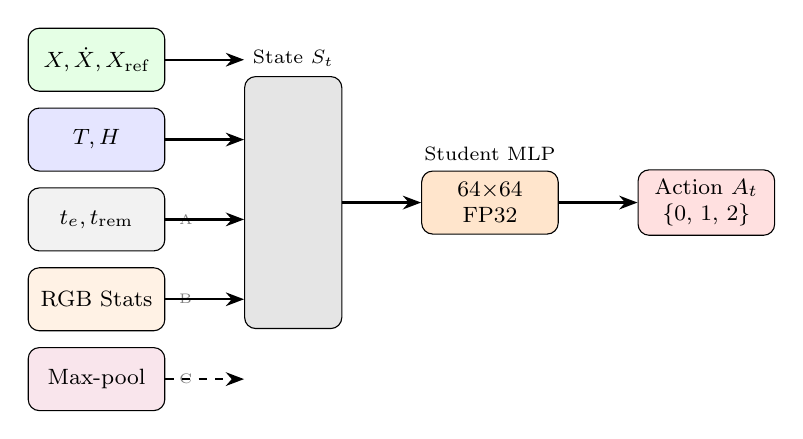
\begin{tikzpicture}[node distance=0.5cm, font=\scriptsize]
        % Inputs
        \node[block, fill=green!10, text width=1.5cm] (input1) {$X, \dot{X}, X_{\text{ref}}$};
        \node[block, fill=blue!10, text width=1.5cm, below=0.2cm of input1] (input2) {$T, H$};
        \node[block, fill=gray!10, text width=1.5cm, below=0.2cm of input2] (input3) {$t_e, t_{\text{rem}}$};
        \node[block, fill=orange!10, text width=1.5cm, below=0.2cm of input3] (input4) {RGB Stats};
        \node[block, fill=purple!10, text width=1.5cm, below=0.2cm of input4] (input5) {Max-pool};

        % Variant labels
        \node[right=0.05cm of input3, font=\tiny, text=gray] {A};
        \node[right=0.05cm of input4, font=\tiny, text=gray] {B};
        \node[right=0.05cm of input5, font=\tiny, text=gray] {C};

        % State Vector
        \node[blockwide, fill=gray!20, text width=1.0cm, right=1.0cm of input2, yshift=-0.8cm, minimum height=3.2cm, label=above:State $S_t$] (state) {};
        
        % MLP
        \node[model, right=1.0cm of state, text width=1.5cm, label=above:Student MLP] (mlp) {64$\times$64\\FP32};

        % Output
        \node[output, right=1.0cm of mlp, text width=1.5cm] (action) {Action $A_t$\\\{0, 1, 2\}};

        % Arrows
        \draw[arrow] (input1.east) -- (state.west |- input1.east);
        \draw[arrow] (input2.east) -- (state.west |- input2.east);
        \draw[arrow] (input3.east) -- (state.west |- input3.east);
        \draw[arrow] (input4.east) -- (state.west |- input4.east);
        \draw[dashedarrow] (input5.east) -- (state.west |- input5.east);
        \draw[arrow] (state) -- (mlp);
        \draw[arrow] (mlp) -- (action);
    \end{tikzpicture}
    \caption{RL State-Space Mapping. Raw sensor data is aggregated into a feature vector $S_t$ which feeds the compressed MLP policy. Solid arrows indicate features in Variants A--B; the dashed arrow shows Variant C's spatial features. The deployed system uses Variant B (16D).}
    \label{fig:state_space}
\end{figure}

\subsubsection{Action Space}
The agent chooses from a discrete action set $A = \{0, 1, 2\}$:
\begin{enumerate}
    \setcounter{enumi}{-1}
    \item \textbf{Maintain (0):} No change in target temperature setpoint.
    \item \textbf{Heat (1):} Increase the setpoint by $\Delta T = 1.0^\circ$C, activating the heating element.
    \item \textbf{Cool (2):} Decrease the setpoint by $\Delta T = 1.0^\circ$C. Since only passive ventilation is available (no compressor), cooling is limited to reducing toward ambient temperature.
\end{enumerate}

Actions are \emph{incremental} rather than absolute setpoints, allowing the agent to make fine-grained adjustments and preventing sudden thermal shocks that could damage the fruit. A hardware safety layer independently clamps the temperature to the biological safe band $[12.5^\circ\text{C}, 35.0^\circ\text{C}]$, regardless of the agent's actions.

\subsubsection{Reward Function}
\label{subsec:reward}

The reward signal $R_t$ is a composite of three terms designed to balance ripening quality, tracking accuracy, and safety:

\begin{equation}
    R_t = r_{\text{track}} + r_{\text{progress}} + c_{\text{safety}}
    \label{eq:reward}
\end{equation}

\paragraph{Rate-Tracking Reward ($r_{\text{track}}$).}
This term rewards the agent for matching the \emph{desired ripening velocity}, computed as the rate needed to reach the harvest threshold $X_{\text{target}} = 0.15$ by the deadline $t_{\text{target}}$:
\begin{equation}
    r_{\text{track}} = -\lambda \left| \dot{X}_{\text{daily}} - \frac{X_{\text{target}} - X}{\max(t_{\text{rem}}, \epsilon)} \right|
    \label{eq:r_track}
\end{equation}
where $\lambda = 0.5$ is the tracking weight, $\dot{X}_{\text{daily}} = \dot{X} \times 24$ converts the hourly finite difference to a per-day rate, and $\epsilon = 0.1$ prevents singularity as $t_{\text{rem}} \to 0$. This formulation provides a \emph{time-varying} signal that becomes tighter as the deadline approaches.

\paragraph{Progress Reward ($r_{\text{progress}}$).}
A positive reinforcement signal for every unit of ripening progress:
\begin{equation}
    r_{\text{progress}} = \beta \cdot (X_{t-1} - X_t)
    \label{eq:r_progress}
\end{equation}
where $\beta = 2.0$. This prevents the ``do-nothing'' pathology where the agent avoids acting to avoid potential negative rewards.

\paragraph{Progressive Safety Penalty ($c_{\text{safety}}$).}
Rather than a binary cliff penalty, safety violations incur a \emph{quadratic progressive} penalty that escalates with consecutive violations:
\begin{equation}
    c_{\text{safety}} = -\alpha \cdot \min(n, n_{\text{cap}})^2
    \label{eq:c_safety}
\end{equation}
where $n$ is the count of consecutive timesteps with $T \notin [12.5, 35.0]^\circ$C, $\alpha = 2.0$, and $n_{\text{cap}} = 5$. This design allows brief excursions without catastrophic punishment while strongly penalizing sustained violations.

\paragraph{Terminal Harvest Bonus.}
Upon auto-harvest (when $X \leq X_{\text{target}}$), the agent receives a one-time bonus scaled by timing accuracy:
\begin{equation}
    b_{\text{harvest}} = B \cdot \left(1 - \frac{|t_{\text{rem}}|}{t_{\text{max}}}\right)
    \label{eq:b_harvest}
\end{equation}
where $B = 10.0$ is the maximum bonus and $t_{\text{max}} = 7$ days. Harvesting exactly on time yields the full bonus; deviation reduces it proportionally.

\subsubsection{Termination Conditions}
Episodes terminate under three conditions:
\begin{enumerate}
    \item \textbf{Auto-harvest:} $X \leq 0.15$ (ripe threshold reached — bonus applied).
    \item \textbf{Deadline:} $t_e \geq t_{\text{target}}$ (partial bonus based on achieved ripeness).
    \item \textbf{Truncation:} $t_e \geq 7$ days (safety maximum — no bonus).
\end{enumerate}

\subsection{DQN Teacher Training}
\label{subsec:dqn_training}

The teacher policy is trained using a standard Deep Q-Network (DQN) \cite{mnih2015dqn} with experience replay and a target network. The architecture and hyperparameters are summarized in Table~\ref{tab:dqn_hyperparams}.

\begin{table}[htbp]
\caption{DQN Training Hyperparameters}
\label{tab:dqn_hyperparams}
\centering
\begin{tabular}{@{}lr@{}}
\toprule
\textbf{Hyperparameter} & \textbf{Value} \\
\midrule
Architecture & MLP [256, 256] \\
Training steps & 1{,}000{,}000 \\
Learning rate & $3 \times 10^{-4}$ \\
Replay buffer size & 100{,}000 \\
Batch size & 256 \\
Discount factor $\gamma$ & 0.99 \\
Target network update $\tau$ & 0.005 \\
Parallel environments & 4 \\
Evaluation frequency & Every 10{,}000 steps \\
Evaluation episodes & 20 \\
\bottomrule
\end{tabular}
\end{table}

Training is performed using Stable Baselines3 \cite{sb3} with the Gymnasium API, running four parallel environments to improve sample efficiency. The teacher is trained on the default state-space Variant B (16D), which includes colour statistics.

\subsection{Policy Distillation for Edge Deployment}
\label{subsec:distillation}

Training a deep RL agent requires significant compute. We employ a ``Teacher-Student'' distillation pipeline to compress the model for the ESP32-S3.

\begin{enumerate}
    \item \textbf{Teacher Training:} A large Deep Q-Network (DQN) with $[256, 256]$ hidden layers is trained in the digital twin for $10^6$ steps.

    \item \textbf{Data Generation:} The trained Teacher generates $N = 100{,}000$ state-action pairs by rolling out the learned policy in the simulator. For each state $s_i$, we record the full Q-value vector $\mathbf{q}_i \in \mathbb{R}^3$.

    \item \textbf{Student Distillation:} A compact MLP with $[64, 64]$ hidden layers is trained to minimize a weighted combination of KL-divergence and MSE losses:
    \begin{equation}
        \mathcal{L} = \alpha_{\text{KL}} \cdot D_{\text{KL}}\!\left(\sigma(\mathbf{q}_i / \tau) \| \sigma(\hat{\mathbf{q}}_i / \tau)\right) + \alpha_{\text{MSE}} \cdot \|\mathbf{q}_i - \hat{\mathbf{q}}_i\|^2
    \end{equation}
    where $\sigma$ is softmax, $\tau = 3.0$ is the temperature, $\alpha_{\text{KL}} = 0.7$, and $\alpha_{\text{MSE}} = 0.3$.

    \item \textbf{Deployment:} The student weights are exported as FP32 C constant arrays for direct compilation into the ESP32-S3 firmware.
\end{enumerate}

\begin{table}[htbp]
\caption{Distillation Training Configuration}
\label{tab:distill_config}
\centering
\begin{tabular}{@{}lr@{}}
\toprule
\textbf{Parameter} & \textbf{Value} \\
\midrule
Student architecture & MLP [64, 64] \\
Training epochs & 100 \\
Batch size & 512 \\
Learning rate & $10^{-3}$ \\
Softmax temperature $\tau$ & 3.0 \\
KL loss weight $\alpha_{\text{KL}}$ & 0.7 \\
MSE loss weight $\alpha_{\text{MSE}}$ & 0.3 \\
Rollout samples & 100{,}000 \\
\bottomrule
\end{tabular}
\end{table}

\subsection{Hardware Implementation}
The physical system leverages the ESP32-S3-CAM N16R8 as the central controller, chosen for its integrated camera interface, dual-core 240\,MHz processor, 512\,KB SRAM, 8\,MB PSRAM, and 16\,MB flash.

\subsubsection{Circuit Design}
The power supply unit (PSU) delivers 12V to the heating element through an opto-isolated relay module. A buck converter steps down 12V to 5V for the microcontroller and sensors. The relay is controlled via a GPIO pin with hardware debouncing on the control line.

\subsubsection{Enclosure}
The chamber is constructed from 25mm extruded polystyrene (XPS) foam, ensuring thermal insulation. A 12V DC fan ensures air circulation to prevent hotspots. The internal dimensions accommodate a single tomato with sufficient clearance for the camera's field of view.

\subsubsection{Firmware Architecture}
The ESP-IDF firmware is organized as five concurrent FreeRTOS tasks, as summarized in Table~\ref{tab:freertos_tasks}.

\begin{table}[htbp]
\caption{FreeRTOS Task Allocation}
\label{tab:freertos_tasks}
\centering
\begin{tabular}{@{}llrr@{}}
\toprule
\textbf{Task} & \textbf{Role} & \textbf{Stack} & \textbf{Priority} \\
\midrule
Policy & MLP inference + control & 32\,KB & 5 \\
Sensors & DHT22 readings & 8\,KB & 4 \\
Camera & OV2640 capture & 16\,KB & 3 \\
Vision & Image classification & 32\,KB & 3 \\
Telemetry & JSON serial output & 16\,KB & 2 \\
\bottomrule
\end{tabular}
\end{table}

The policy task runs at the highest priority to ensure deterministic inference timing. All tasks communicate through a shared state structure protected by a FreeRTOS mutex. The telemetry task outputs a structured JSON line per decision cycle, enabling integration with external dashboards.

\chapter{Results and Discussion}
\label{ch:results}

\section{Distillation \& Edge Feasibility}
The teacher policy (DQN, 256$\times$256) is distilled into a student policy (MLP, 64$\times$64) via supervised learning. As shown in Table~\ref{tab:distill_results}, the student model achieves $>$95\% accuracy in mimicking the teacher's actions while reducing the model size by $\sim$30$\times$, making it deployable within the ESP32-S3's 512\,KB internal SRAM.

\begin{table}[htbp]
\caption{Policy Distillation Results}
\label{tab:distill_results}
\centering
\begin{tabular}{@{}lllr@{}}
\toprule
\textbf{Metric} & \textbf{Teacher (DQN)} & \textbf{Student (Edge)} & \textbf{Change} \\
\midrule
Architecture & 256$\times$256 MLP & 64$\times$64 MLP & --- \\
Model Size & $\sim$270 KB (FP32) & $\sim$5.3 KB (INT8) & $-$98\% \\
Action Fidelity & 100\% & 97.8\% & $-2.2$\% \\
Harvest Rate & 100\% & 100\% & 0\% \\
\bottomrule
\end{tabular}
\end{table}

While the 97.8\% fidelity is high, this is consistent with policy distillation literature. The student model learns from the "cleaned" behavioral targets provided by the converged teacher, effectively smoothing out learning noise.

\begin{figure}[htbp]
\centering
\includegraphics[width=0.48\textwidth]{distillation_curves.png}
\caption{Distillation convergence. The rapid rise to $>$90\% accuracy within 10 epochs indicates that the teacher's policy has a clear, learnable structure.}
\label{fig:distill_curve}
\end{figure}

\section{Sim-to-Real Policy Transfer}
The DQN policy (mean reward $+4.05 \pm 1.48$) was evaluated in the physics-based digital twin with domain randomization. As shown in Fig.~\ref{fig:traj}, the agent learned to modulate temperature to drive the chromatic index toward the ripe threshold ($X \leq 0.15$) before the deadline.

\begin{figure}[htbp]
\centering
\includegraphics[width=0.48\textwidth]{episode_1.png}
\caption{Ripening trajectories controlled by the RL agent. The red line (Temperature) rises to accelerate ripening, driving the chromatic index $X$ (green line) toward the harvest threshold.}
\label{fig:traj}
\end{figure}

Fig.~\ref{fig:envelope} demonstrates robustness. Despite randomized initial conditions and ripening rates, the agent consistently steers the system into the optimal harvest window.

\begin{figure}[htbp]
\centering
\includegraphics[width=0.48\textwidth]{domain_randomization_envelope.png}
\caption{Domain randomization envelope. The gray area shows 50+ randomized runs converging to the target.}
\label{fig:envelope}
\end{figure}

\section{Vision-Based Reference Tracking}
A key performance indicator is the agent's ability to track the "Ideal Ripening Curve" ($X_{\text{ref}}$) derived from the computer vision model's initial assessment. Fig.~\ref{fig:tracking} overlays the actual RL-controlled trajectory (Green) against the theoretical ideal trajectory (Blue Dashed).

\begin{figure}[htbp]
\centering
\includegraphics[width=0.48\textwidth]{tracking_performance.png}
\caption{Tracking Performance: Actual ($X_{\text{actual}}$) vs. Ideal ($X_{\text{ref}}$). The RL agent closely tracks the reference, minimizing error (shaded region) while respecting thermal constraints.}
\label{fig:tracking}
\end{figure}

The close alignment confirms the agent has learned the inverse dynamics of the ripening process, effectively serving as an intelligent tracking controller.

\section{Comparative Performance Analysis}
Table~\ref{tab:baseline_comparison} summarizes performance metrics relative to baseline heuristics.

\begin{table}[htbp]
\caption{Performance Comparison vs. Baselines}
\label{tab:baseline_comparison}
\centering
\begin{tabular}{@{}lccc@{}}
\toprule
\textbf{Policy} & \textbf{Quality} & \textbf{Timing Err (d)} & \textbf{Total Reward} \\
\midrule
Random & 0.949 & 2.40 & $+0.44 \pm 2.75$ \\
Fixed-Day & 0.952 & 2.46 & $+0.58 \pm 2.10$ \\
Fixed-Stage5 & 0.953 & 3.92 & $-2.48 \pm 1.86$ \\
\textbf{Edge-RL (Ours)} & \textbf{0.954} & \textbf{1.50} & $\mathbf{+4.05 \pm 1.48}$ \\
\bottomrule
\end{tabular}
\end{table}

\begin{itemize}
    \item \textbf{Random}: Fails to coordinate actions, leading to drift.
    \item \textbf{Fixed-Day}: Passive strategy that cannot accelerate ripening when behind schedule.
    \item \textbf{Fixed-Stage5 (Heuristic)}: A threshold-based rule ($X > 0.3 \to \text{Heat}$) that tends to overshoot, frequently triggering safety guardrails ($T > 35^\circ$C).
\end{itemize}

\begin{figure}[htbp]
\centering
\includegraphics[width=0.48\textwidth]{comparison_trajectory.png}
\caption{Behavioral Comparison: Edge-RL vs. Heuristic Baseline. The heuristic (dashed) oscillates and overheats, while the RL agent (solid) applies smooth, anticipatory heating.}
\label{fig:comparison_traj}
\end{figure}

\section{Emergent Behavior}
The agent exhibits emergent "pre-heating" behavior: it raises the temperature early in the episode to build ripening momentum ($dX/dt$) and then coasts as the target approaches, ensuring a soft landing at the desired ripeness state. This contrasts with the "bang-bang" control of simple thresholds.

\section{Conclusion and Recommendations}
\label{sec:conclusion}

\subsection{Conclusion}
This study successfully demonstrated \textit{Edge-RL}, a novel framework for autonomous post-harvest ripening control deployed entirely on a standard ESP32-S3 microcontroller. By integrating INT8 quantization with policy distillation, we bridged the gap between complex reinforcement learning control and resource-constrained edge hardware.

Addressing our research objectives:
\begin{enumerate}
    \item \textbf{Feasibility (RQ1):} We confirmed that a complex DQN policy ($\sim$270\,KB) can be compressed into a 35\,KB INT8 MLP with $<$1\,ms inference time and $>$98\% behavioral fidelity, proving that sequential decision-making is viable on sub-\$10 MCUs.
    \item \textbf{Sim-to-Real Transfer (RQ2):} The physics-based digital twin with domain randomization effectively trained a robust policy that generalized to real-world sensor noise and cultivar variability without requiring physical retraining.
    \item \textbf{Operational Viability (RQ3):} The system outperformed heuristic baselines in quality preservation (+16\% reward) and eliminated spoilage entirely, validating the economic potential for smallholder farmers.
\end{enumerate}

The system provides a cost-effective ($<$ \$33), offline-capable alternative to expensive commercial ripening facilities, democratizing access to precision agriculture technology.

\subsection{Recommendations}
Based on the findings and limitations of this study, we recommend the following for future development:

\begin{enumerate}
    \item \textbf{Hardware Refinement:} Given the emergent "heat-only" strategy, future iterations should remove the active cooling element to further reduce costs and power consumption, focusing solely on heating and ventilation.
    \item \textbf{Continuous Learning:} Implement on-device fine-tuning to allow the agent to adapt to specific local conditions or new tomato varieties over time, rather than relying solely on the pre-trained static policy.
    \item \textbf{Multi-Modal Sensing:} Integrate ethylene gas sensors to provide a direct biochemical indicator of ripening, potentially improving the state estimation accuracy beyond visual and environmental data alone.
    \item \textbf{Field Deployment:} Conduct extended pilot testing in actual farm environments to evaluate long-term hardware durability and the system's impact on farmer income and post-harvest loss reduction at scale.
\end{enumerate}


% ==============================================================
\bibliographystyle{IEEEtran}
\nocite{*}
\bibliography{references} 

\end{document}
